%%%%%%%%%%%%%%%%%%%%%%%%%%%%% Define Article %%%%%%%%%%%%%%%%%%%%%%%%%%%%%%%%%%
\documentclass{article}
%%%%%%%%%%%%%%%%%%%%%%%%%%%%%%%%%%%%%%%%%%%%%%%%%%%%%%%%%%%%%%%%%%%%%%%%%%%%%%%

%%%%%%%%%%%%%%%%%%%%%%%%%%%%% Using Packages %%%%%%%%%%%%%%%%%%%%%%%%%%%%%%%%%%
\usepackage{geometry}
\usepackage{graphicx}
\usepackage{amssymb}
\usepackage{amsmath}
\usepackage{amsthm}
\usepackage{empheq}
\usepackage{mdframed}
\usepackage{booktabs}
\usepackage{lipsum}
\usepackage{graphicx}
\usepackage{color}
\usepackage{psfrag}
\usepackage{pgfplots}
\usepackage{bm}
%%%%%%%%%%%%%%%%%%%%%%%%%%%%%%%%%%%%%%%%%%%%%%%%%%%%%%%%%%%%%%%%%%%%%%%%%%%%%%%

% Other Settings

%%%%%%%%%%%%%%%%%%%%%%%%%% Page Setting %%%%%%%%%%%%%%%%%%%%%%%%%%%%%%%%%%%%%%%
\geometry{a4paper}

%%%%%%%%%%%%%%%%%%%%%%%%%% Define some useful colors %%%%%%%%%%%%%%%%%%%%%%%%%%
\definecolor{ocre}{RGB}{243,102,25}
\definecolor{mygray}{RGB}{243,243,244}
\definecolor{deepGreen}{RGB}{26,111,0}
\definecolor{shallowGreen}{RGB}{235,255,255}
\definecolor{deepBlue}{RGB}{61,124,222}
\definecolor{shallowBlue}{RGB}{235,249,255}
%%%%%%%%%%%%%%%%%%%%%%%%%%%%%%%%%%%%%%%%%%%%%%%%%%%%%%%%%%%%%%%%%%%%%%%%%%%%%%%

%%%%%%%%%%%%%%%%%%%%%%%%%% Define an orangebox command %%%%%%%%%%%%%%%%%%%%%%%%
\newcommand\orangebox[1]{\fcolorbox{ocre}{mygray}{\hspace{1em}#1\hspace{1em}}}
%%%%%%%%%%%%%%%%%%%%%%%%%%%%%%%%%%%%%%%%%%%%%%%%%%%%%%%%%%%%%%%%%%%%%%%%%%%%%%%

%%%%%%%%%%%%%%%%%%%%%%%%%%%% English Environments %%%%%%%%%%%%%%%%%%%%%%%%%%%%%
\newtheoremstyle{mytheoremstyle}{3pt}{3pt}{\normalfont}{0cm}{\rmfamily\bfseries}{}{1em}{{\color{black}\thmname{#1}~\thmnumber{#2}}\thmnote{\,--\,#3}}
\newtheoremstyle{myproblemstyle}{3pt}{3pt}{\normalfont}{0cm}{\rmfamily\bfseries}{}{1em}{{\color{black}\thmname{#1}~\thmnumber{#2}}\thmnote{\,--\,#3}}
\theoremstyle{mytheoremstyle}
\newmdtheoremenv[linewidth=1pt,backgroundcolor=shallowGreen,linecolor=deepGreen,leftmargin=0pt,innerleftmargin=20pt,innerrightmargin=20pt,]{theorem}{Theorem}[section]
\theoremstyle{mytheoremstyle}
\newmdtheoremenv[linewidth=1pt,backgroundcolor=shallowBlue,linecolor=deepBlue,leftmargin=0pt,innerleftmargin=20pt,innerrightmargin=20pt,]{definition}{Definition}[section]
\theoremstyle{myproblemstyle}
\newmdtheoremenv[linecolor=black,leftmargin=0pt,innerleftmargin=10pt,innerrightmargin=10pt,]{problem}{Problem}[section]
%%%%%%%%%%%%%%%%%%%%%%%%%%%%%%%%%%%%%%%%%%%%%%%%%%%%%%%%%%%%%%%%%%%%%%%%%%%%%%%

%%%%%%%%%%%%%%%%%%%%%%%%%%%%%%% Plotting Settings %%%%%%%%%%%%%%%%%%%%%%%%%%%%%
\usepgfplotslibrary{colorbrewer}
\pgfplotsset{width=8cm,compat=1.9}
%%%%%%%%%%%%%%%%%%%%%%%%%%%%%%%%%%%%%%%%%%%%%%%%%%%%%%%%%%%%%%%%%%%%%%%%%%%%%%%

%%%%%%%%%%%%%%%%%%%%%%%%%%%%%%% Title & Author %%%%%%%%%%%%%%%%%%%%%%%%%%%%%%%%
\title{Apuntes de practicas}
\author{Rodrigo Miranda}
%%%%%%%%%%%%%%%%%%%%%%%%%%%%%%%%%%%%%%%%%%%%%%%%%%%%%%%%%%%%%%%%%%%%%%%%%%%%%%%

\begin{document}
    \maketitle
    Ejemplos de practica AMN941  - Usando Latex en VSCode
    \section*{Punto Fijo}
    \subsection*{Ejemplo 1}Use el método de punto para encontrar una raíz real de la ecuación
    \[
        f(x)= x^{3}+2x^{2}+10x-20 =0
        \]
    Empleando como valor inicial $x0=1$. Emplee $15$ decimales y una precisión de $10^{-5}$.


    \textbf{Solucion:} 

    \noindent Para punto fijo, debemos obtener una ecuacion $g(x)=x$ 


    \textbf{Opcion 1:} $x= x^{3}+2x^{2}+11x-20$
    
    \noindent \\ Verificamos que la ecuacion converga en el punto dado, para ello derivamos la ecuacion $g(x)$ y evaluamos en el punto, de manera que:

    $g'(x)=3x^{2}+4x+11 \longrightarrow g'(1)=18$

    \noindent \\ Esto lo podemos comprobar rapidamente tambien en matlab, de la siguiente manera
    \begin{figure}[ht]
        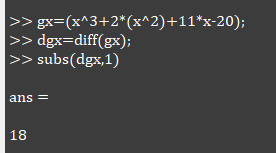
\includegraphics[scale=1]{img/ejemplo_clasePunto.png}
        \caption[Derivada y evaluacion g'(x)]{Matlab 1}
    \end{figure}
    \\Por lo tanto, incumplimos el teorema de Banach quien expresa que $|g'(x)|<1$ \pagebreak
    
    \textbf{Opcion 2: }$\frac{20}{x^2+2x+10}$
    \noindent \\Probamos esta ecuacion y derivada evaluada en matlab
    \begin{figure}[ht]
        \includegraphics*[scale=0.9]{img/ejemplo_clasePunto_2.png}
        \caption[Derivada y evaluacion g'(x)]{Matlab 2}
    \end{figure}
    \\Como podemos observar, el resultado de la evaluacion es menor a 1, por lo tanto si converge.

    \noindent Probaremos esta ecuacion con el metodo de punto fijo en Matlab.
    \begin{figure}[ht]
        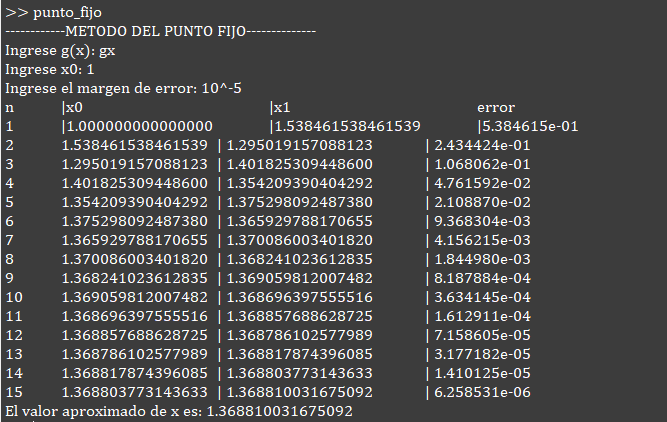
\includegraphics[scale=0.8]{img/ejemplo_clasePunto_3.png}
        \caption[Metodo Punto Fijo]{Matlab 3}
    \end{figure}
    \\El valor aproximado de $x=1.368810031675092$


    \section*{Newton}
    \subsection*{Ejemplo 1}
    Use el método de Newton - Raphson para encontrar una solución exacta con una exactitud de $10^{-12}$ para la siguiente ecuación. Emplee 15 decimales: 
    \[
        \ln(x-1)+cos(x-1)=0 ; [1.3,2]
    \]
    \begin{figure}[ht]
        \includegraphics*[scale=0.9]{img/ejemplo3.png}
    \end{figure}
    
    \textbf{Nota:} Cuando estemos trabajando ejercicios, es importante analizar la grafica. Dado que no podemo modificar la ecuacion como en el metodo de punto fijo, debemos elegir correctamente nuestro valor inicia,
    para esto, debemos alegarnos de: Puntos de infleccion, maximos y minimos relativos y extremos, en estas partes no nos funcionara este metodo.
    Ademas, si la primera derivada de la ecuacion es 0, no nos funcionara este metodo.
\pagebreak
\section*{Metodo de la Secante}
La diferencia principal de este metodo es que necesitamos de dos valores iniciales x0 y x1, este nos formara dos puntos.  \textbf{Secante exige que la ecuacion
este de la forma f(x)=0}
\subsection*{Ejemplo 1} Se tienen dos postes, uno de 29 pies de altura y otro de 41 pies de altura, los  cuales están separados entre si 47 pies. Los postes se sostienen mediante dos cables, conectados a una sola
estaca entre ellos, desde el nivel del suelo hasta la parte superior de cada poste. Emplee el metodo de la secante para determinar donde debe colocarse la estaca, para que la cantidad de cable utilizado sea de 85 pies.
Use una precisión de $10^-12$. Emplee 15 decimales.
\begin{figure}[ht]
    \includegraphics*[scale=0.9]{img/secante0.png}
\end{figure}
\noindent \\¿De donde vienen estas raices? Bueno, si aplicamos pitagoras de acuerdo a la información que tenemos gracias al ejercicio (marcadas en azul en la imagen), podemos obtener cada uno de los catetos o hipotenusas
que representan los otros lados de los triangulos.

\noindent \\ Sabemos que la suma del todal del cable utilizado debe ser 85, y conocemos la ecuacion gracias a pitagoras que me permite plantear cuando deberian valer esos segmentos de cable.
Por tanto, podemos plantear esa ecuacion de la siguiente forma

\noindent \\ $\sqrt[]{29^2+(47-x)^2}+\sqrt[]{x^2+41^2}=85$
\\$f(x)=\sqrt[]{29^2+(47-x)^2}+\sqrt[]{x^2+41^2}-85$
\pagebreak
\noindent Grafiquemos para entender
\begin{figure}[ht]
    \includegraphics*[scale=0.55]{img/secante01.png}
\end{figure}

\noindent \\ Como observamos, es una ecuacion cuadratica que corta en dos puntos al eje X.
\\Vamos a operar en matlab eligiendo dos puntos cercanos a la primera raiz, en este caso usaremos: [20,22]
\begin{figure}[ht]
    \includegraphics*[scale=0.7]{img/secante02.png}
    \\ \includegraphics*[scale=0.8]{img/secante03.png}
\end{figure}
\noindent \\El resultado de la primera raiz es de 21.065779178000248
\\Ahora trabajaremos con  la otra raiz, para eso utilizarmemos los puntos [33,34]
\begin{figure}[ht]
    \includegraphics*[scale=0.7]{img/secante04.png}
\end{figure}

\pagebreak
\subsection*{Ejemplo 2}
\begin{figure}[ht]
    \includegraphics*[scale=0.9]{img/ej20_secante.png}
\end{figure}
\subsection*{Calculando tiempo en el que llega a su altura maxima}Iniciemos determinando su altura maxima.

\noindent $\mathbf{V}y(t) = 0$\indent   En su punto mas alto
\\Hace falta recordar que: La ecuacion de velocidad, la podemos obtener encontrando la derivada de le ecuacion de la posicion vertical.
\\Tal que: $\mathbf{V}y(t)=\partial y(t)=(CVy = 9.8C^2)(\frac{e^\frac{-t}{c}}{c})-9.8C$

$f(x)=(CVy + 9.8C^2)(\frac{e^\frac{-t}{c}}{c})-9.8C=0$

\noindent \\Declaremos las variables en Matlab:

$
ang=57.82\\
v0=3925\\
m=159.09\\
k=9.5\\ 
vx=v0*cosd(57.82)\\ 
vy=v0*sind(ang)\\
c=\frac{m}{k}
$

\noindent Ahora, debemos identificar el intervalo donde esta la raiz, por lo que procedemos a graficar la funcion en Matlab
\begin{figure}[ht]
    \includegraphics*[scale=0.7]{img/secante05.png}
    \\ \includegraphics*[scale=0.7]{img/secante06.png}
\end{figure}
\noindent \\ Observando, notamos que el intervalo de la raiz, donde el eje x corta la funcion, es entre 51 y 52. Usamos el metodo en Matlab
\begin{figure}[ht]
    \includegraphics*[scale=0.7]{img/secante07.png}
\end{figure}
\\Ahora conocemos el tiempo en el que llega a su altura maxima, que es de: 51.176626309310990. Encontremos su altura maxima:
\begin{figure}[ht]
    \includegraphics*[scale=1]{img/secante08.png}
\end{figure}

\subsection*{Calculando el tiempo que tarda en llegar al suelo}
Para determinar el tiempo que tarda en llegar al suelo, podemos partir de: Cuando el objeto toca el suelo $h_m=0$ y $v=0$ 
\\Por tanto: $g(x)=(c*vy+9.8*c^2)*(1-exp(-x/c))-9.8*c*x=0$. Un tiempo 0 no haria sentido, tampoco uno negativo, por lo que debemos graficar la funcion en valores separados para encontrar su raiz, tal que:
\begin{figure}[ht]
    \includegraphics*[scale=0.5]{img/secante09.png}
\end{figure}

Obseravamos que la raiz se encuentra entre 350 y 360. Procedemos a ejcutar secante. 
\begin{figure}[ht]
    \includegraphics*[scale=0.7]{img/secante10.png}{\\ Encontramos el tiempo que se tarda en tocar el suelo $t=355.729791053669490$}
\end{figure}

\pagebreak
\subsection*{Encontrando el alcance horizontal}
Cnocemos el tiempo que se tarda en caer nuevamente el objeto, por lo tanto, sustituyendo este tiempo en la funcion de desplazamiento en X podemos 
encontrar el alcance horizontal.
\begin{figure}[ht]
    \includegraphics*[scale=0.6]{img/secante11.png}
\end{figure}

\pagebreak
\section*{Metodo de la posicion falsa}
\textbf{Ejemplo:} Se construye una caja sin tapadera a partir de una hoja metalica rectangular que mide 150 por 115 centimentros. Cual debe ser el lad de los cuadrados que hay que recortar en cada esquina para que
el volumen de la caja se de 50,601. 6875 centimentros cubicos? Precision de $10^{12}$. Emplee el metodo de la posicion falsa. Use 15 decimales.

\begin{figure}[ht]
    \includegraphics*[scale=1]{img/secante1.png}
\end{figure}

\noindent $\mathbb{V} = 50,601.6875$
\\$\mathbb{V} = l.h.a$
\\$\mathbb{V} = (150-2x).(115.2x)$
\\$50,601.6875 = (150-2x).(115-2x).x$

\textbf{Nota: }\\Metodo de posicion falsa requiere un $f(x)=0$
\\ $f(x)=(150-2x).(115-2x).x-50,601.6875=0$

\begin{figure}[ht]
    \includegraphics*[scale=0.5]{img/secante2.png}
\end{figure}
Observando la grafica en geogebra, identificamos que la funcion tiene 3 raices. Para saber cual de ellas nos puede servir, debemos ocupar la logica.
\begin{itemize}
    \item ¿Hace sentido una pestaña de altura entre 3 y 4 cm? Si, hace sentido.
    \item ¿Hace sentido una pestaña entre 45 y 50 cm? Quedaria alta, pero aun asi hace sentido, debemos probar.
    \item ¿Hace sentido una pestaña de mas de 80 cm? La verdad es que no, no nos daria el volumen con pestañas tan altas.
\end{itemize}

Para la primera raiz utilizaremos el intervalo [3,4]
\pagebreak
\section*{Metodo de Steffensen}
\subsection*{Ejemplo 1}
\begin{figure}[ht]
    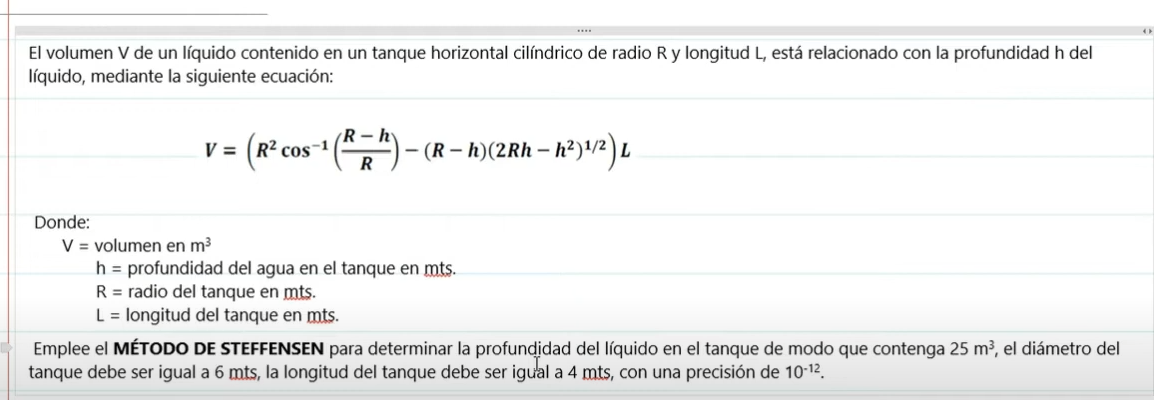
\includegraphics[scale=0.5]{img/stf1.png}
\end{figure}
Iniciamos trabajando la funcion F(x) = 0, para poder graficar y obtener el intervalo que ocuparemos.

$f(x)=(r^2\arccos(\frac{r-h}{r})-(r-h)(2rh-h^2)^0.5)l-v=0$
\begin{figure}[ht]
    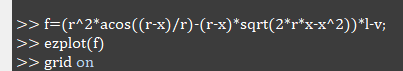
\includegraphics[scale=0.7]{img/stf2.png}
    \\ 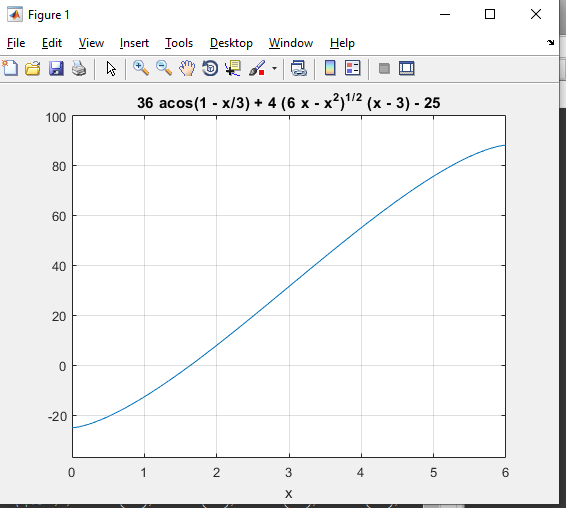
\includegraphics[scale=0.6]{img/stf3.png}{\\Podemo elegir un punto inicial x=1 o el intervalo [1,2]}
\end{figure}
\\Para continuar, el metodo de Steffensen nos pide encontrar g(x)=x, por lo tanto despejamos en nuestra ecuacion:
$x=(r^2\arccos(\frac{r-h}{r})-(r-h)(2rh-h^2)^0.5)l-v+x\\
g(x)=(r^2\arccos(\frac{r-h}{r})-(r-h)(2rh-h^2)^0.5)l-v+x
$

Probemos si este despeje nos funciona, vamos a Matlab: $g=(r^2*acos((r-x)/r)-(r-x)*sqrt(2*r*x-x^2))*l-v+x$
\begin{figure}[ht]
    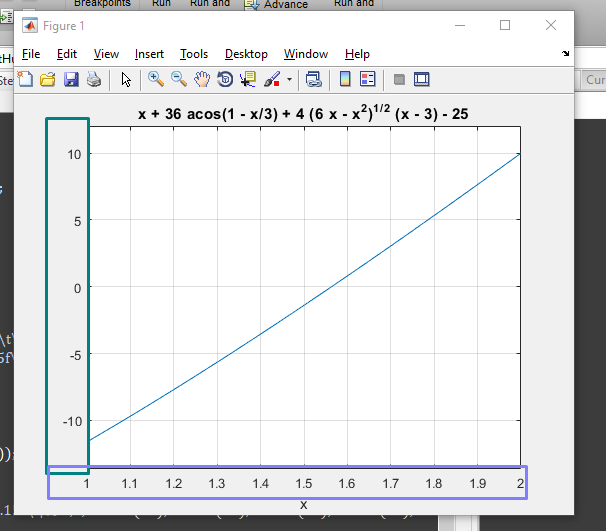
\includegraphics[scale=0.7]{img/stf4.png}{\\Debemos observar detenidamente el grafico, para cumplir el metodo \textbf{los valores en x Y y deben ser iguales}, sin embargo, vemos que para un x=1,y=-10; por lo tanto se separan y por mucho}
    \end{figure}

Debemos corregirlo, y para ello debemos hacer otro despeje. Esta vez intentaremos multiplicando X a ambos lados de la expresion, por lo tanto:
$g(x)=\frac{(r^2acos((r-x)/r)-(r-x)\sqrt{2rx-x^2})lx}{v}$

En matlab:$g=(r^2*acos((r-x)/r)-(r-x)*sqrt(2*r*x-x^2))*l*x/v$
\\Observemos la grafica ahora 
\pagebreak
\begin{figure}[ht]
    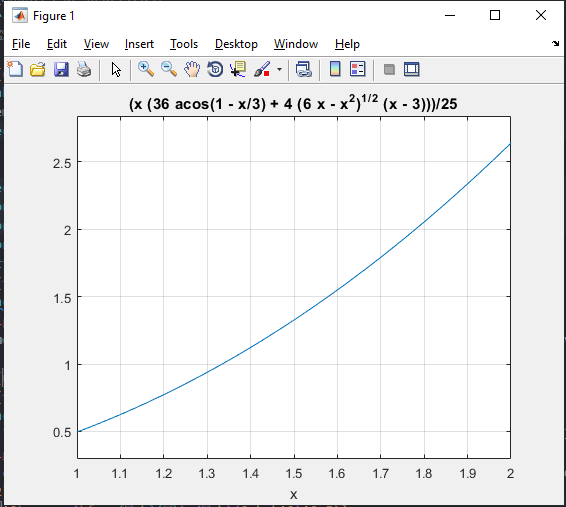
\includegraphics[scale=0.8]{img/stf5.png}{\\Los valores siguen separados, pero esta vez por menos, si observamos para un x=1, y=0.5; por lo tanto podria funcionar.}
\end{figure}
\\Sin embargo, debemos buscar un mejor valor inicial [1,2] ya no nos sirve. Revisemos nuevamente el grafico de la funcion f(x)=0 para
encontrar un mejor intervalo.Para ello, la graficamos exactamene en ese intervalo que ahora estamos descartando.
\begin{figure}[ht]
    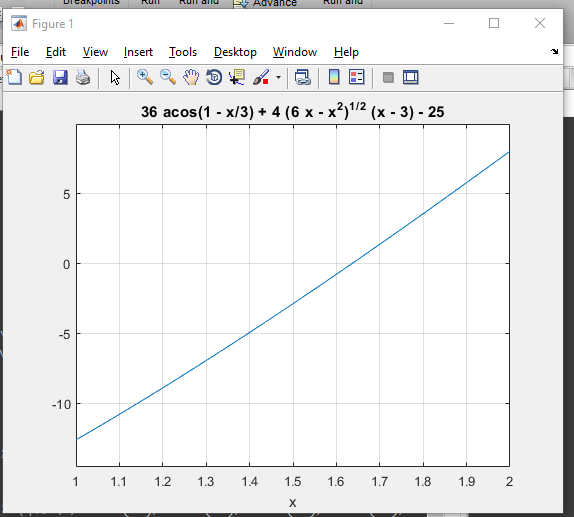
\includegraphics[scale=0.8]{img/stf6.png}{\\Con un valor de x=1.6 podria converger rapidamente. Recordemos, buscamos el punto donde corta el eje x}
\end{figure}

El resultado es el siguiente:
\begin{figure}[ht]
    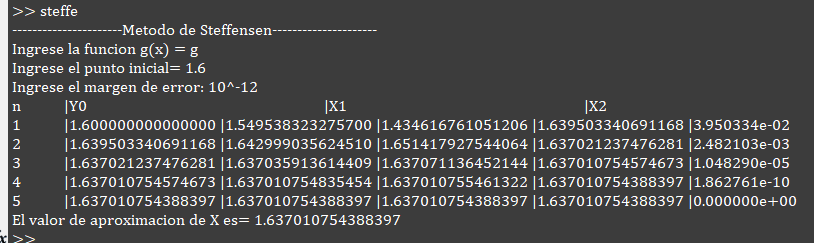
\includegraphics[scale=0.7]{img/stf7.png}{\\La profundidad del liquido es: h=1.637010754388397}
\end{figure}


\end{document}